\section{Introduction}

%Intro
Gravitational lensing and dynamical modelling provide independent constraints on the mass distribution of galaxies. Combining them allows for valuable cross-checking opportunities to resolve degeneracies inherent in both methods. It can also help to disentangle the stellar and dark matter content of galaxies.

%Dark Matter
The flat rotation curves of galaxies \citep{1978ApJ...225L.107R} were the first indication that galaxies might reside in massive, almost spherical halos made of invisible ``dark'' matter. The standard model of cosmology, based on results by the Planck Mission \citep{WMAP5cosm} \Wilma{[TO DO: Aaron thinks Dunkley is a WMAP paper.... Check difference WMAP/Planck...]}, infers that $\sim 85\%$ of the universe's total matter content is in the form of non-baryonic cold dark matter. Simulations suggest that this kind of dark matter forms cuspy halos following a Navarro-Frenk-White (NFW) profile \citep{NFW96}. However, central dark matter density cusps are not observed in dark matter dominated dwarf galaxies (e.g., \citealt{1994Natur.370..629M,2001ApJ...552L..23D}). Their existence in more massive galaxies depends strongly on stellar mass-to-light ratio (e.g., \citealt{2011MNRAS.416..322D}). Overall, observations suggest cored dark matter halos. This discrepancy, known as the core-cusp problem, might be resolved by galaxy formation processes such as mergers and outflows (e.g., \citealt{2001ApJ...560..636E,2012MNRAS.421.3464P}).

Determining the overall mass distribution in massive galaxies and separating the dark from the stellar mass components is therefore a crucial step in better understanding the structure of galaxies and nature or dark matter.

%Lensing
Strong gravitational lensing is an independent method to tightly constrain the projected total mass of galaxies inside $\sim 1''$. Massive galaxies can act as gravitational lenses and deflect the light of background sources, giving rise to multiple distorted images of the source. By 2010 over 200 strong gravitational galaxy lenses had been discovered and the number is still rising (e.g., \citealt{2010ARA&A..48...87T}).

%Dynamical modelling
The mass profile at larger galactocentric radii can be probed by gas rotation curves that directly measure the galaxy's circlar velocity profile \Wilma{[TO DO: REF]}. However, due to its dissipative nature, gas motions are very sensitive to disturbances by e.g. spiral arms and bars \Wilma{[TO DO: REF]}.

Because stars are dissipationless dynamical tracers and present almost everywhere in the galaxy, stellar dynamical modelling can complement mass constraints from lensing at small and gas motions at large radii. But stellar motions are complex: a bulk rotation around one principal axis combined with random motions in all coordinate direction. Full dynamical modelling of rotation, dispersion and velocity anisotropies is needed to deduce the matter distribution.

The Sloan WFC Edge-on Late-type Lens Survey (SWELLS, WFC = Wide field camera) \citep{SWELLSI,SWELLSII,SWELLSIII,SWELLSIV,SWELLSV,SWELLSVI} is dedicated to find and investigate spiral galaxies, seen almost edge-on so rotation curves can be easily measured, that are also strong gravitational lenses. By combining lensing and dynamical modelling degeneracies inherent in both methods can be broken. SWELLS picked galaxies in SDSS whose spectra had two different redshifts within $3''$, which makes it likely to capture strong lenses with typical Einstein radii of $1''$. Sufficiently inclined galaxies were picked by eye. Follow up high resolution imaging with the Hubble Space Telescope's (HST) Wide-Field Planetary Camera 2 (WFPC2) was performed to confirm their lensing status \citep{SWELLSI}.

%Characteristics of J1331
One of the SWELLS galaxies is SDSS J1331+3628, to which we refer as J1331 in the remainder of this work. It is a spiral galaxy of approximate Hubble type Sb at right ascension = 202.91800$^\circ$ and a declination = 36.46999$^\circ$ (epoch J2000). It has bluish spiral arms and a large reddish bulge (see Figures \ref{fig:F450W} and \ref{fig:F814W}), which is superimposed by quadruplet of extended bluish images approximately at a distance of $1''$ from the galaxy center (see Figure \ref{fig:lens_just_imgpos}). The lensed object might be a star-forming blob of a background galaxy. J1331 stands out of the SWELLS sample because of its large counter-rotating core (see Figure \ref{fig:kinematics}), which might be an indication that J1331 underwent a minor merger in its recent past.

%Previous results
\citet{SWELLSI} confirmed that J1331 was a strong gravitational lens, measured its apparent brightness and estimated the stellar masses of disk and bulge. The lensing properties of J1331 were first analysed by \citet{SWELLSIII}. \citet{SWELLSV} measured the gas and stellar kinematics along the major axis and deduced J1331's mass profile from the gas rotation curve at large radii and total mass inside the Einstein radius from gravitational lensing, focusing mostly on the outer regions of J1331.

%Goal of this work
The goal of this work is to complement the previous work on J1331 by an in-depth analysis of the matter distribution in J1331's inner regions. We use stellar dynamical modelling in addition to lensing constraints, similar to a study of the Einstein Cross by \citet{GlennEC}. We attempt to disentangle the stellar and dark matter components and test if employed axisymmetric Jeans models work also in the presence of a counter-rotating core. Ideally this work on J1331 could also help understanding how minor mergers modify the mass distribution of a galaxy.

This paper is organized as follows: Section \ref{sec:Modelling} gives an overview of the modelling techniques used in this work, Section \ref{sec:data} summarizes the data and Section \ref{sec:Results} presents our results on the surface photometry of J1331 using Multi-Gaussian expansions (Section \ref{sec:MGE_results}), constraints from lensing (Section \ref{sec:results_lensing}) and Jeans modelling based on the surface brightness only (Section \ref{sec:results_JAM_SB}) and including a NFW dark matter halo (Section \ref{sec:results_JAM_NFW}). Finally Section \ref{sec:Discussion} uses the result to discuss J1331's stellar mass-to-light ratio and possible merger history and starting points for future work.

%\paragraph{Methods}
%\begin{itemize}
%\item lensing: fitting scale-free galaxy model to image positions \citep{EvansWitt}
%\item photometry: MGE expansion of surface brightness in the F814W filter (deconvolution with PSF), apparent magnitude, total luminosity, effective radius
%\item Jeans modelling: jeans axisymmetric modelling (JAM) by \citet{Cap08} to fit model predictions for the second velocity moments to the stellar kinematics data
%\end{itemize}


%============================================================================


\begin{figure*}
\centering
\begin{subfigure}{.5\textwidth}
  \centering
  \includegraphics[width=.9\linewidth]{fig/first_glimpse_450.ps}
  \caption{J1331 in F450W}
  \label{fig:F450W}
\end{subfigure}%
\begin{subfigure}{.5\textwidth}
  \centering
  \includegraphics[width=.9\linewidth]{fig/first_glimpse_814.ps}
  \caption{J1331 in F814W}
  \label{fig:F814W}
\end{subfigure}
\begin{subfigure}{.5\textwidth}
  \centering
  \includegraphics[width=.9\linewidth]{fig/lens_imgpos.ps}
  \caption{The lensing images}
  \label{fig:lens_just_imgpos}
\end{subfigure}%
\begin{subfigure}{.5\textwidth}
  \centering
  \includegraphics[width=.9\linewidth]{fig/stellar_kinematics_data.ps}
  \caption{Stellar Kinematics by \citet{SWELLSV}}
  \label{fig:kinematics}
\end{subfigure}
\caption{Hubble Space telescope (HST) images and stellar kinematics of the galaxy SDSS J1331+3628 (J1331), which has a large counter-rotating core and whose bulge acts as a strong lens for a bluish background source. \emph{Panel (a) and (b):} HST/WFPC2/WFC3 images of J1331 by \citet{SWELLSI} in two filters, F450W in panel (a) and F814W in panel (b). The galaxy's coordinates on the sky are right ascension $\alpha$ = 202.91800$^\circ$ and declination $\delta$ = 36.46999$^\circ$ (epoch J2000). Image orientation and scaling are indicated in panel (a); the scaling transformation from arcseconds to the physical size of the galaxy in kpc uses the galaxy's redshift $z_d = 0.113$ \citep{SWELLSIII} (i.e. assumes an angular diameter distance of 414 Mpc). The color scaling of these two images is the same. The black solid line in panel (b) shows the orientation of the major-axis. The line has a length of $10''$ and indicates the region within which we carry out the Jeans modelling. \emph{Panel (c):} The central region of J1331 in F450W, surface brightness subtracted. An IRAF \emph{ellipse} fit to the F450W surface brightness in panel (a) was subtracted from the image. The (smoothed) residuals within the white square in panel (a) are shown in panel (c). Four bright blobs (A,B,C and D) become visible, which are arranged in a typical strong lensing configuration around the center of the galaxy (G). \emph{Panel (d):} Stellar Kinematics along the galaxy's major axis as measured by \citet{SWELLSV}, line-of-sight rotation velocity $v_\text{rot}$, line-of-sight velocity dispersion $\sigma$ and the rms-velocity $v_\text{rms} = \sqrt{v_\text{rot}^2 + \sigma^2}$. The dotted line in panel (b) indicates the galaxy's effective half-light radius (in the F814W filter), $R_\text{eff} = 2.6" = 5.2$ kpc. The $v_\text{rot}$ curve reveals that J1331 is counter-rotating within $R_\text{eff}$. \Wilma{[TO DO: Replace arcsec with '' in panel d)]} \Wilma{[TO DO: Mention, that the configuration of the additional two bright blobs do not suggest that they form a lensing doublet. They are probably background star formation regions as well. The blob above A could be stretched due to lensing and have a faint counter image between B and G. Maybe indicate in plot?]}}
\label{fig:specialJ1331}
\end{figure*}